\documentclass[aspectratio=169,14pt,usenames,dvipsnames]{beamer}
\usetheme{TalentSprint}
\usepackage[utf8]{inputenc}
\usepackage{graphics}
\usepackage{ragged2e}
\usepackage{amsfonts}
\usepackage{xcolor}
\usepackage{mathtools}
\usepackage{tcolorbox}
\usepackage{setspace}
\usepackage{lmodern}
\definecolor{swe}{rgb}{0.19, 0.73, 0.56}
\definecolor{lgreen}{RGB}{190,200,198}
\title[Keras]{Keras}


\begin{document}

{\1
\begin{frame} \vspace{35pt}
%	\title[Keras]{Keras}
	\subtitle{Deep Learning Framework}
	\maketitle
\end{frame}
}


\begin{frame}{What is Keras?}

\begin{itemize}
\item Deep neural network library in Python
\begin{itemize}
\item High-level neural networks API
\item Modular – Building model is just stacking layers 
\item Runs on top of either TensorFlow
\end{itemize}
\end{itemize}
\end{frame}

\begin{frame}{What is Keras? (Cont..)}
\begin{itemize}
\item Why use Keras ?

\begin{itemize}
\item Useful for fast prototyping, ignoring the details of implementing backprop or
\item writing optimization procedure
\item Supports Convolution, Recurrent layer and combination of both.
\item Runs seamlessly on CPU and GPU
\item Almost any architecture can be designed using this framework
\item Open-Source code – Large community support

\end{itemize}
\end{itemize}

Documentation: \underline{\url{http://keras.io/}}

\end{frame}

\begin{frame}{Three API styles (Keras Models)}
\begin{itemize}
\item The Sequential Model
\begin{itemize}
\item Dead simple
\item Only for single-input, single-output, sequential layer stacks
\item Allows you to create models layer-layer by stacking them
\end{itemize}
\end{itemize}

\begin{itemize}
\item The functional API
\begin{itemize}
\item Flexible model architecture (each layer can be connected in a pairwise fashion).
\item Multi-input, multi-output, arbitrary static graph topologies
\item Can create complex network such as Residual Network.

\end{itemize}
\end{itemize}
\end{frame}


\begin{frame}{Three API styles (Keras Models) (Cont...)}
\begin{itemize}
\item Model subclassing
\begin{itemize}
\item More Flexible than Functional or Sequential.
\item arger potential error surface
\end{itemize}
\end{itemize}

\end{frame}

\begin{frame}{Keras Sequential model}
\begin{itemize}
\item The Sequential model is a linear stack of layers
\item You can create a Sequential model by passing a list of layer instances to the constructor:
\end{itemize}
\centering
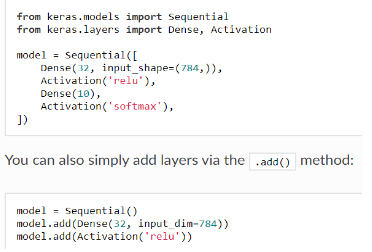
\includegraphics[width=0.45\textwidth, height=0.45\textheight]{Keras_Images/Ker_1.png}
\end{frame}

\begin{frame}{The functional API}
\centering

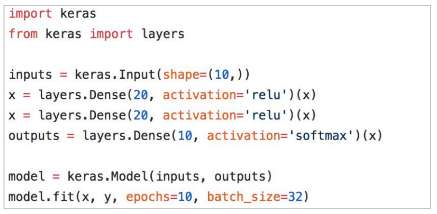
\includegraphics[width=0.55\textwidth, height=0.45\textheight]{Keras_Images/Ker_2.png}
\end{frame}

\begin{frame}{Model subclassing}
\centering
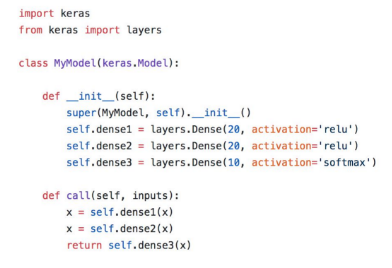
\includegraphics[width=0.55\textwidth, height=0.6\textheight]{Keras_Images/Ker_3.png}
\end{frame}

\begin{frame}{Sequential model – steps}
\begin{columns}
\column{0.6\textwidth}
\begin{itemize}
\item \textbf{Specifying the input shape}
\begin{itemize}
\item Input\_shape
\item Input\_dim
\end{itemize}
\end{itemize}

\begin{itemize}
\item \textbf{Compiling}
\begin{itemize}
\item Optimizer
\item Loss function
\item Metrics
\end{itemize}
\end{itemize}

\begin{itemize}
\item \textbf{Training}
\begin{itemize}
\item Optimizer
\item Loss function
\item Metrics
\end{itemize}
\end{itemize}


\column {0.6\textwidth}
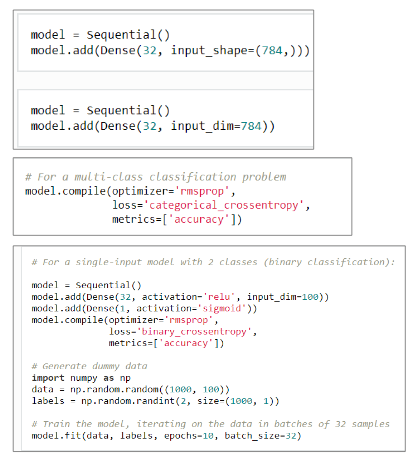
\includegraphics[width=6cm, height=5.5cm]{Keras_Images/Ker_4.png}
\end{columns}
\end{frame}


\begin{frame}{Model parameters}
\begin{itemize}
\item Neural Network Model Parameters
\begin{itemize}
\item No. of neurons in each layer
\item Connection between neurons from different layers
\item Activation Function
\item Optimization Method
\item Error Function
\end{itemize}
\end{itemize}

\end{frame}

\begin{frame}{Model parameters (Cont..)}
\begin{itemize}
\item Training (Time) Parameter
\begin{itemize}
\item No of epochs
\item Batch size
\end{itemize}
\end{itemize}

\begin{itemize}
\item Evaluation
\begin{itemize}
\item Measurement
\item Training/Validation/Test
\end{itemize}
\end{itemize}

\end{frame}

\begin{frame}{Handwriting Digit Recognition}
\begin{center}
\only<1->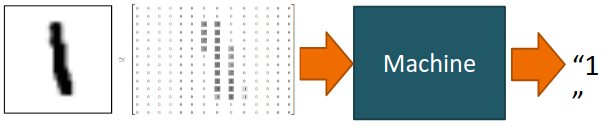
\includegraphics[width=9cm, height=2.5cm]{Keras_Images/Ker_5.png} \\
\item<2-> MNIST Data: \underline{\url{http://yann.lecun.com/exdb/mnist/}}\\
\end{center}
\end{frame}


\begin{frame}{Handwriting Digit Recognition}
\begin{center}
\only<1->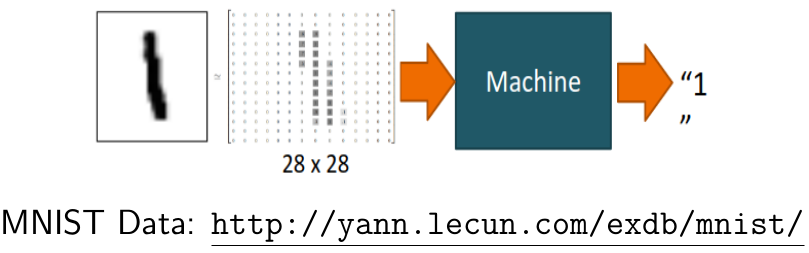
\includegraphics[width=12cm, height=4cm]{Keras_Images/Ker_6.png} \\
\item<2-> Keras provides data sets loading function: \underline{\url{http://keras.io/datasets/}}\\
\end{center}
\end{frame}

\begin{frame}{Keras: Building a Network}
\centering

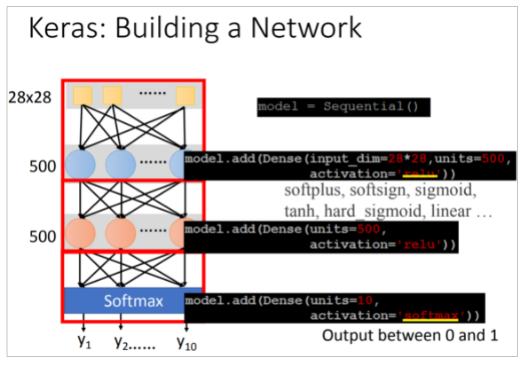
\includegraphics[width=7cm, height=5.5cm]{Keras_Images/Ker_7.png}
\end{frame}

\begin{frame}
\centering

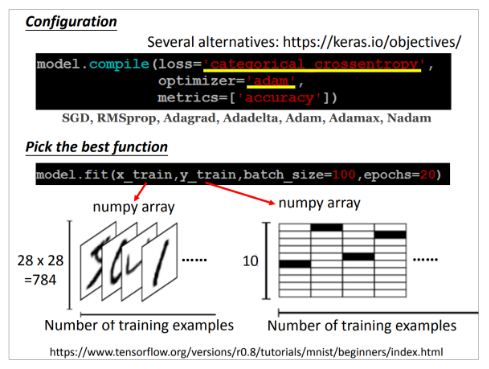
\includegraphics[width=8cm, height=6cm]{Keras_Images/Ker_8.png}
\end{frame}


\begin{frame}{Keras}
          \begin{columns}
                \begin{column}{0.6\textwidth}
			\begin{itemize}
				\item<1-> Save and load models 
				\item<2-> How to use the neural network (testing):
				\item<3-> 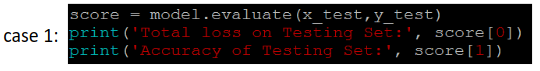
\includegraphics[width=1.0\textwidth, height=0.1\textheight]{Keras_Images/Ker_10.png}
				\item<4-> 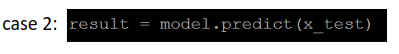
\includegraphics[width=0.6\textwidth, height=0.1\textheight]{Keras_Images/Ker_11.png}
			\end{itemize}
                        
                \end{column}
                \begin{column}{0.5\textwidth}
			\vspace{0.5cm}
			\begin{overlayarea}{0.9\textwidth}{0.5\textheight}
			\only<1>{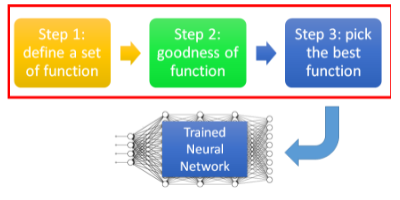
\includegraphics[width=0.9\textwidth, height=0.5\textheight]{Keras_Images/Ker_9.png}}
			\only<2>{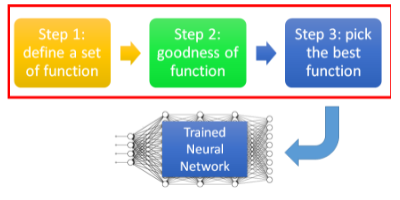
\includegraphics[width=0.9\textwidth, height=0.5\textheight]{Keras_Images/Ker_9.png}}
\only<3-4>{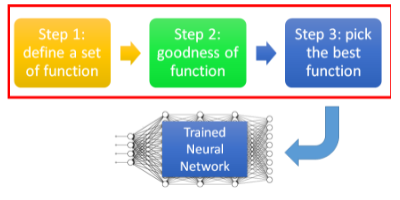
\includegraphics[width=0.9\textwidth, height=0.5\textheight]{Keras_Images/Ker_9.png}}


			\end{overlayarea}
                \end{column}
        \end{columns}
\end{frame}


\begin{frame}{Example: Estimate the price \\ of a house based on its attributes.}
\centering

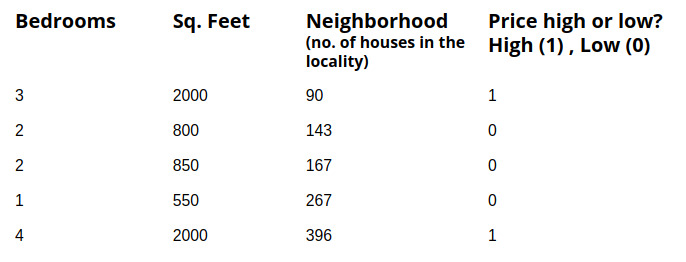
\includegraphics[width=9.5cm, height=4.5cm]{Keras_Images/Ker_12.png}
\end{frame}

\begin{frame}{MLP Architecture}
\centering

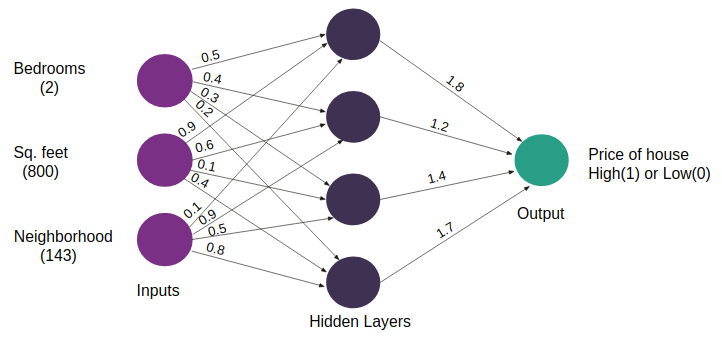
\includegraphics[width=9cm, height=5cm]{Keras_Images/Ker_13.png}
\end{frame}


\begin{frame}{MLP Architecture}

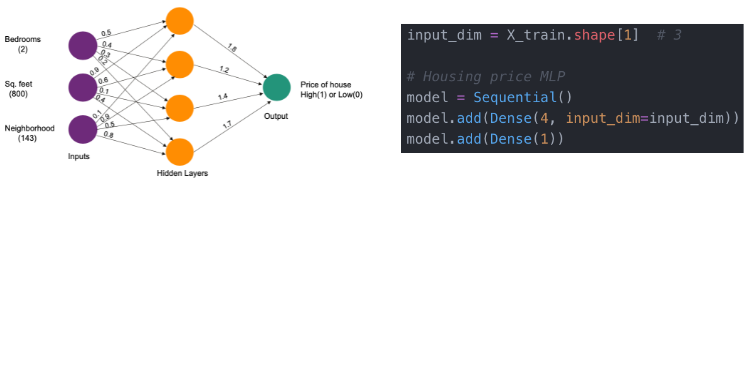
\includegraphics[width=14.5cm, height=6cm]{Keras_Images/Ker_14.png}

\end{frame}

\begin{frame}{MLP Architecture : output as sigmoid }

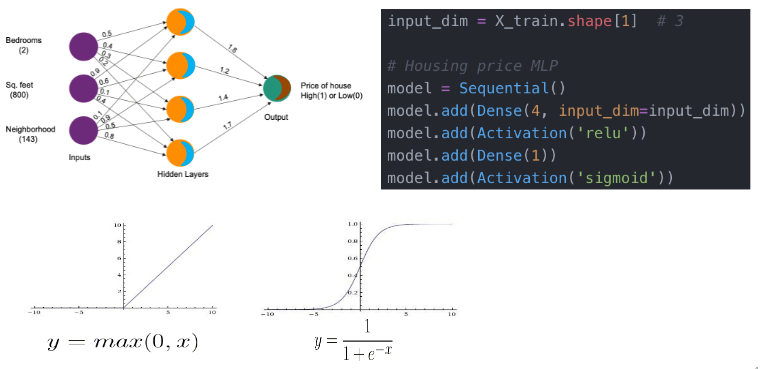
\includegraphics[width=14.5cm, height=6cm]{Keras_Images/Ker_15.png}

\end{frame}

\begin{frame}{MLP Architecture : output as one-hot encoded class}

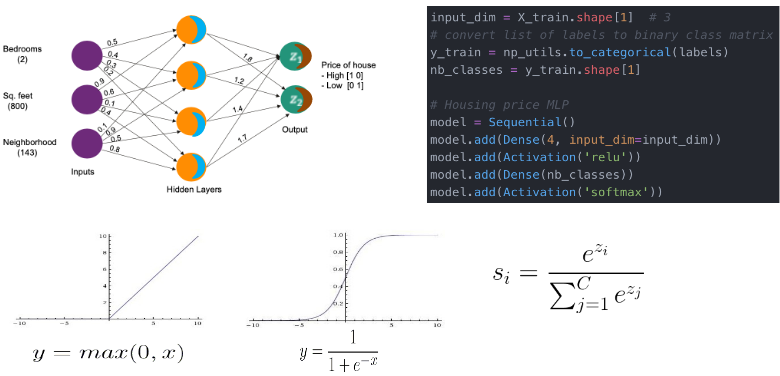
\includegraphics[width=14.5cm, height=6cm]{Keras_Images/Ker_16.png}

\end{frame}

\begin{frame}{Loss / Objective}

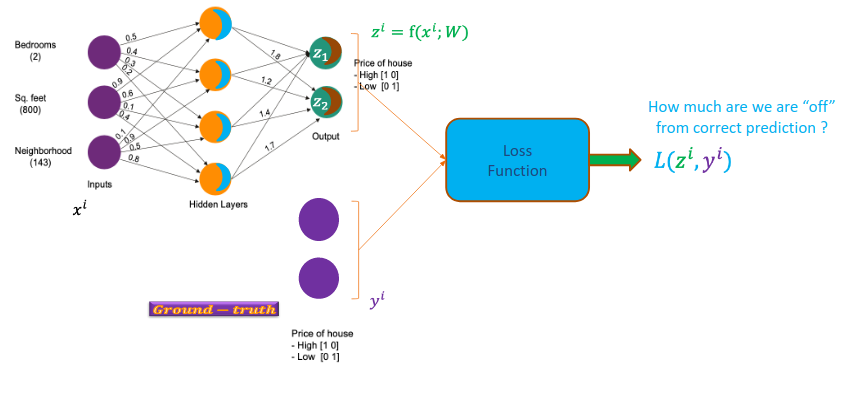
\includegraphics[width=14.5cm, height=6cm]{Keras_Images/Ker_17.png}

\end{frame}


\begin{frame}{Loss / Objective}

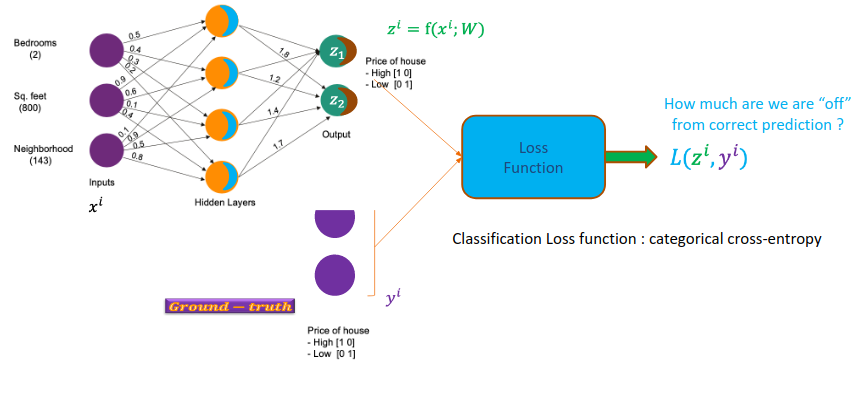
\includegraphics[width=14.5cm, height=6cm]{Keras_Images/Ker_18.png}

\end{frame}

\begin{frame}{Loss / Objective}

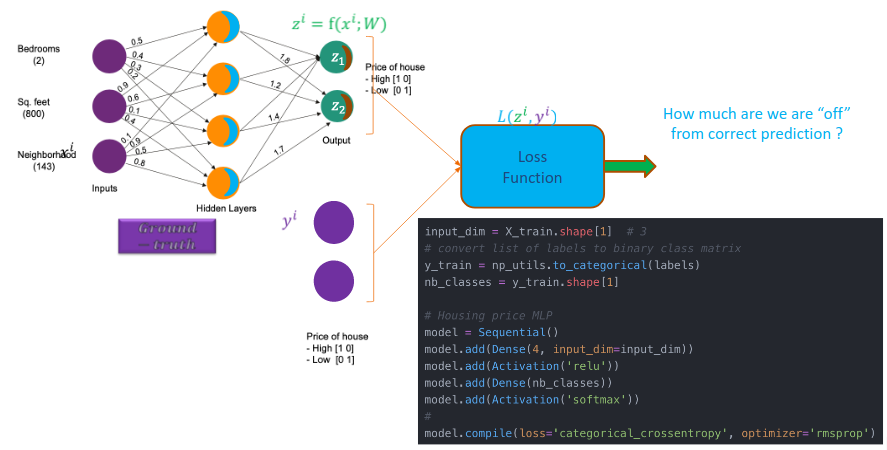
\includegraphics[width=14.5cm, height=6cm]{Keras_Images/Ker_19.png}

\end{frame}


\begin{frame}{Backpropagation}

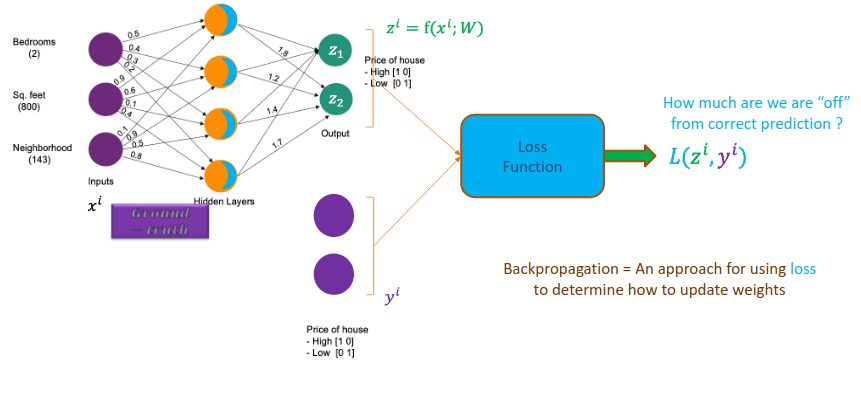
\includegraphics[width=14.5cm, height=6cm]{Keras_Images/Ker_20.png}

\end{frame}


\begin{frame}

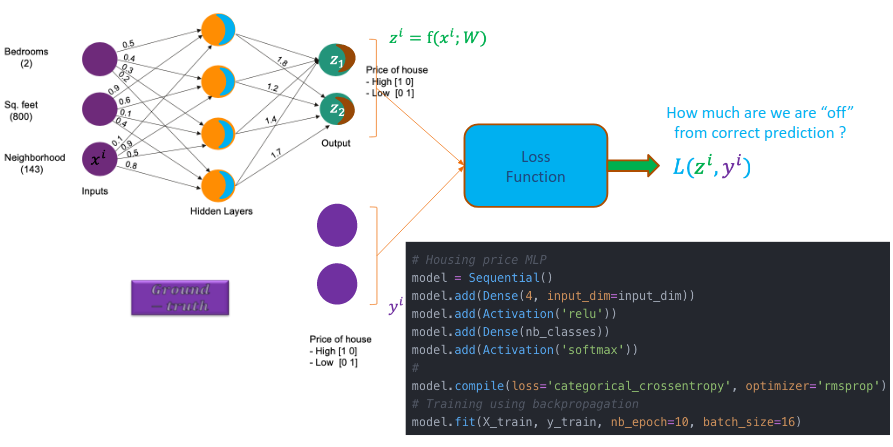
\includegraphics[width=14.5cm, height=6cm]{Keras_Images/Ker_21.png}

\end{frame}


\begin{frame}{Measuring Classification Performance}
\centering
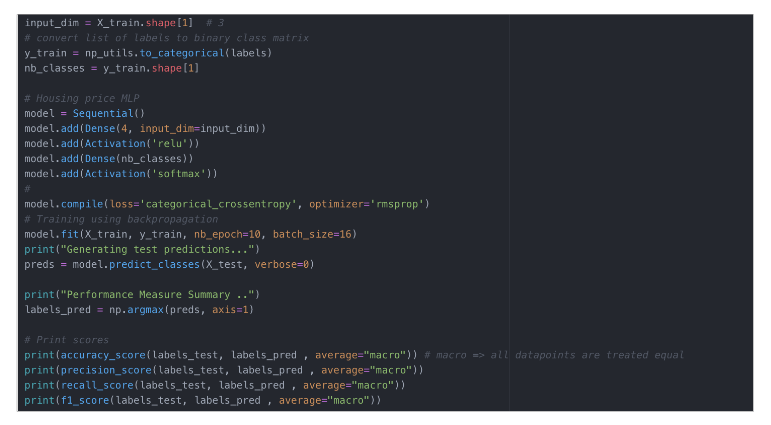
\includegraphics[width=11cm, height=6cm]{Keras_Images/Ker_22.png}

\end{frame}


\begin{frame}{CNN example (CIFAR-10)}
\centering
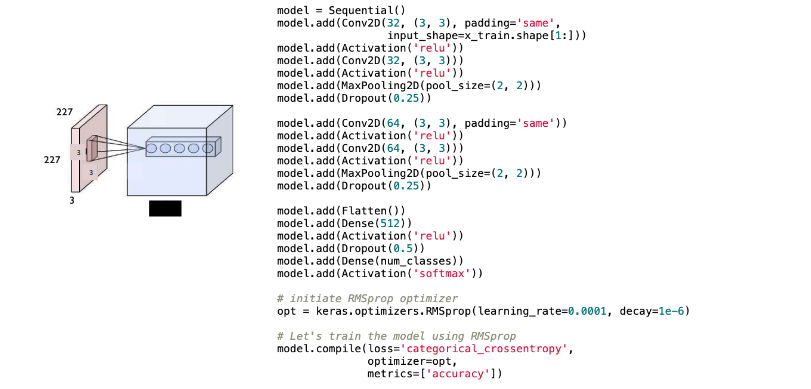
\includegraphics[width=12cm, height=5cm]{Keras_Images/Ker_23.png}

\underline{\url{https://keras.io/examples/cifar10_cnn/}}

\end{frame}


{\1
\begin{frame}
	\title{Thanks!!}
	\subtitle{Questions?}
	\maketitle
\end{frame}}


\end{document}

